In this Chapter we present the software model of \texttt{OpenNN}. 
The whole process is carried out in the Unified Modeling Language (UML).
The final implementation is written in the C++ Programming Language.

\section{Unified Modeling Language (UML)}

The Unified Modeling Language (UML) is a general purpose visual
modeling language that is used to specify, visualize, construct,
and document the artifacts of a software system
\cite{Rumbaugh1999}.

In order to construct a model for \texttt{OpenNN}, we
follow a top-down development. This approach to the problem begins
at the highest conceptual level and works down to the details. In
this way, to create and evolve a conceptual class diagram, we iteratively model:

\begin{enumerate}
\item Classes.
\item Associations.
\item Compositions.
\item Derived classes.
\item Members.
\item Methods.
\end{enumerate}

\section{Classes}\index{class, object oriented programming}

% Introduction

In colloquial terms a concept is an idea or a thing. In
object-oriented modeling concepts are represented by means of
classes \cite{Stroustrup2000}. Therefore, a prime task is to
identify the main concepts (or classes) of the problem domain. In
UML class diagrams, classes are depicted as boxes
\cite{Rumbaugh1999}.

% OpenNN

Through all this work, we have seen that general problemss can be solved 
with three elements: a neural network, a
performance functional and a training strategy. The characterization
in classes of these three concepts for \texttt{OpenNN} is
as follows:

\begin{description}

\item[NeuralNetwork] 

The class representing the concept of neural network is called \lstinline"NeuralNetwork".

\item[Performance functional]

The class which represents the concept of performance functional is called \lstinline"PerformanceFunctional".

\item[Training strategy]

The class representing the concept of training strategy is called \lstinline"TrainingStrategy".

\end{description}

Figure \ref{ConceptDiagram} depicts a starting UML class diagram
for the conceptual model of \texttt{OpenNN}.

\begin{figure}[h!]
\begin{center}
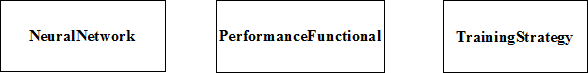
\includegraphics[width=0.975\textwidth]{software_model_basis/concept_diagram}
\caption{Conceptual diagram for \texttt{OpenNN}.}\label{ConceptDiagram}
\end{center}
\end{figure}


\section{Associations}
\index{association, object oriented programming}

% Introduction

Once identified the main concepts in the model it is necessary to
aggregate the associations among them. An association is a
relationship between two concepts which points some significative
or interesting information \cite{Stroustrup2000}. In UML class
diagrams, an association is shown as a line connecting two
classes. It is also possible to assign a label to an association.
The label is typically one or two words describing the association
\cite{Rumbaugh1999}.

% OpenNN

The appropriate associations among the main concepts of \texttt{OpenNN} are next identified to
be included to the UML class diagram of the system:

\begin{description}
\item[Neural network- Performance functional]
A neural network \textit{has assigned} a performance
functional.
\item[Performance functional - Training strategy]
A performance functional \textit{is improved by} a training
strategy.
\end{description}

Figure \ref{AssociationDiagram} shows the above UML class diagram
with these associations aggregated.

\begin{figure}[h!]
\begin{center}
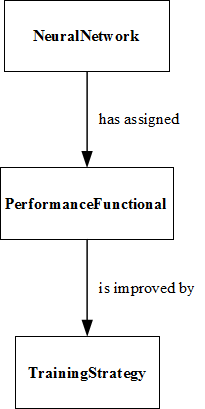
\includegraphics[width=0.35\textwidth]{software_model_basis/association_diagram}
\caption{Aggregation of associations to the conceptual diagram.}\label{AssociationDiagram}
\end{center}
\end{figure}

\section{Composition}

% Introduction

Classes are usually composed of another classes. The higher level classes manage the lower level ones. 

% OpenNN

Regarding \texttt{OpenNN}, the three main concepts described above are quite high level structures. 
This means that the neural network, performance functional and training algorithm classes are composed by different elements. 
In the next chapters the composition of the high level objects is explained in some detail. 

\section{Derived classes}\index{derived class, object oriented programming}

% Introduction

In object-oriented programming, some classes are designed only as
a parent from which sub-classes may be derived, but which is not
itself suitable for instantiation. This is said to be an
\textit{abstract class}\index{abstract class, object oriented
programming}, as opposed to a \textit{concrete
class}\index{concrete class, object oriented programming}, which
is suitable to be instantiated. The derived class contains all the
features of the base class, but may have new features added or
redefine existing features \cite{Stroustrup2000}. Associations
between a base class an a derived class are of the kind \textit{is
a} \cite{Rumbaugh1999}.

% OpenNN

Some \texttt{OpenNN} classes are abstract, and concrete classes are derived from them. 
In the next chapters we will describe the intheritance of the main components 
of \texttt{OpenNN}: the neural network, the performance functional and the training strategy.  

\section{Members and methods} 
\index{attribute, object oriented programming}
\index{operation, object oriented programming}

A member (or attribute) is a named value or relationship that exists for all or some instances of a class. 
A method (or operation) is a procedure associated with a class \cite{Stroustrup2000}. 
In UML class diagrams, classes are depicted as boxes with three sections: the
top one indicates the name of the class, the one in the middle
lists the attributes of the class, and the bottom one lists the
operations \cite{Rumbaugh1999}.

The main members and methodss of the different \texttt{OpenNN} classes are described throughout all this manual. 
